% This is samplepaper.tex, a sample chapter demonstrating the
% LLNCS macro package for Springer Computer Science proceedings;
% Version 2.20 of 2017/10/04
%
\documentclass[runningheads]{llncs}
%
\usepackage{graphicx}
\usepackage{url}
\usepackage[scale=0.70]{geometry}
% Used for displaying a sample figure. If possible, figure files should
% be included in EPS format.
%
% If you use the hyperref package, please uncomment the following line
% to display URLs in blue roman font according to Springer's eBook style:
% \renewcommand\UrlFont{\color{blue}\rmfamily}

\begin{document}
%
\title{Poster proposal: using an online Turing Machine simulator for a theoretical class on complexity and calculability}%\thanks{Supported by ENS Rennes and CentraleSup{\'e}lec.}}
%
\titlerunning{Poster proposal: an online Turing Machine simulator}
% % If the paper title is too long for the running head, you can set
% % an abbreviated paper title here
% %
% \author{Lilian Besson\inst{1}\orcidID{0000-0003-2767-2563}}
% %
% \authorrunning{Lilian Besson}
% % First names are abbreviated in the running head.
% % If there are more than two authors, 'et al.' is used.
% %
% \institute{{\'E}cole Normale Sup{\'e}rieure de Rennes, Bruz, France\\
% \email{lilian.besson{@}ens-rennes.fr}\\
% \url{http://www.ens-rennes.fr/}}
%
\maketitle              % typeset the header of the contribution
%
\begin{abstract}
    % The abstract should briefly summarize the contents of the paper in 150--250 words.
    % https://www.didapro.org/8/contributions-dates/
    I propose a poster which will present an online Turing Machine simulator (\url{https://naereen.github.io/jsTuring_fr/turing.html}),
    which has been used successfully for a course introducing calculability and complexity to engineering students in France,
    as well as for a master's degree course for students preparing the computer science major option at the ``agr{\'e}gation'' national exam in mathematics.
    The poster detail the user interface of the Turing Machine simulator, and explain these two successful use cases.
\keywords{Turing Machine \and Online tool for teaching theoretical computer science \and Javascript \and Open-source tool.}
\end{abstract}
%
%
%

% -------------------------
\section{Outline of the poster content}

The poster will present the following points.

\paragraph{Presentation of Turing Machine}

I quickly introduce the notations of the Turing Machine model, using modern notations \cite{turingmachine}, and not the historical notations from Turing's paper.
%
A (one-tape) Turing machine can be formally defined as a 7-tuple $M=\langle Q,\Gamma ,b,\Sigma ,\delta ,q_{0},F\rangle$ where

\begin{small}
\begin{itemize}
    \item
    $Q$ is a finite, non-empty set of states;
    \item
    $\Gamma$ is a finite, non-empty set of tape alphabet symbols;
    \item
    $b\in \Gamma$ is the blank symbol (the only symbol allowed to occur on the tape infinitely often at any step during the computation);
    \item
    $\Sigma \subseteq \Gamma \setminus \{b\}$ is the set of input symbols, that is, the set of symbols allowed to appear in the initial tape contents;
    \item
    $q_{0}\in Q$ is the initial state;
    \item
    $F\subseteq Q$ is the set of final states or accepting states. The initial tape contents is said to be accepted by $M$ if it eventually halts in a state from $F$.
    \item
    $\delta :(Q\setminus F)\times \Gamma \not \to Q\times \Gamma \times \{L,R\}$ is a partial function called the transition function, where L is left shift, R is right shift. If $\delta$ is not defined on the current state and the current tape symbol, then the machine halts.
\end{itemize}
\end{small}


\paragraph{Presentation of the online Turing Machine simulator}

The presented Turing Machine simulator \cite{morphett_simulators,naereen_simulators},
can be found online at
\url{http://morphett.info/turing/} in English,
and \url{https://naereen.github.io/jsTuring_fr/turing.html} in French.
%
By including two screenshots of the user interface, we present the different components of a Turing Machine (tape, state, input word, transition table etc).
We also present the user interface of the simulator, which allows to save a machine described by its transition table $\delta$ to an online file (using GitHub's anonym gists, \url{https://gist.github.com/}), and to load machines already written.

\begin{figure}[!h]
    \centering
    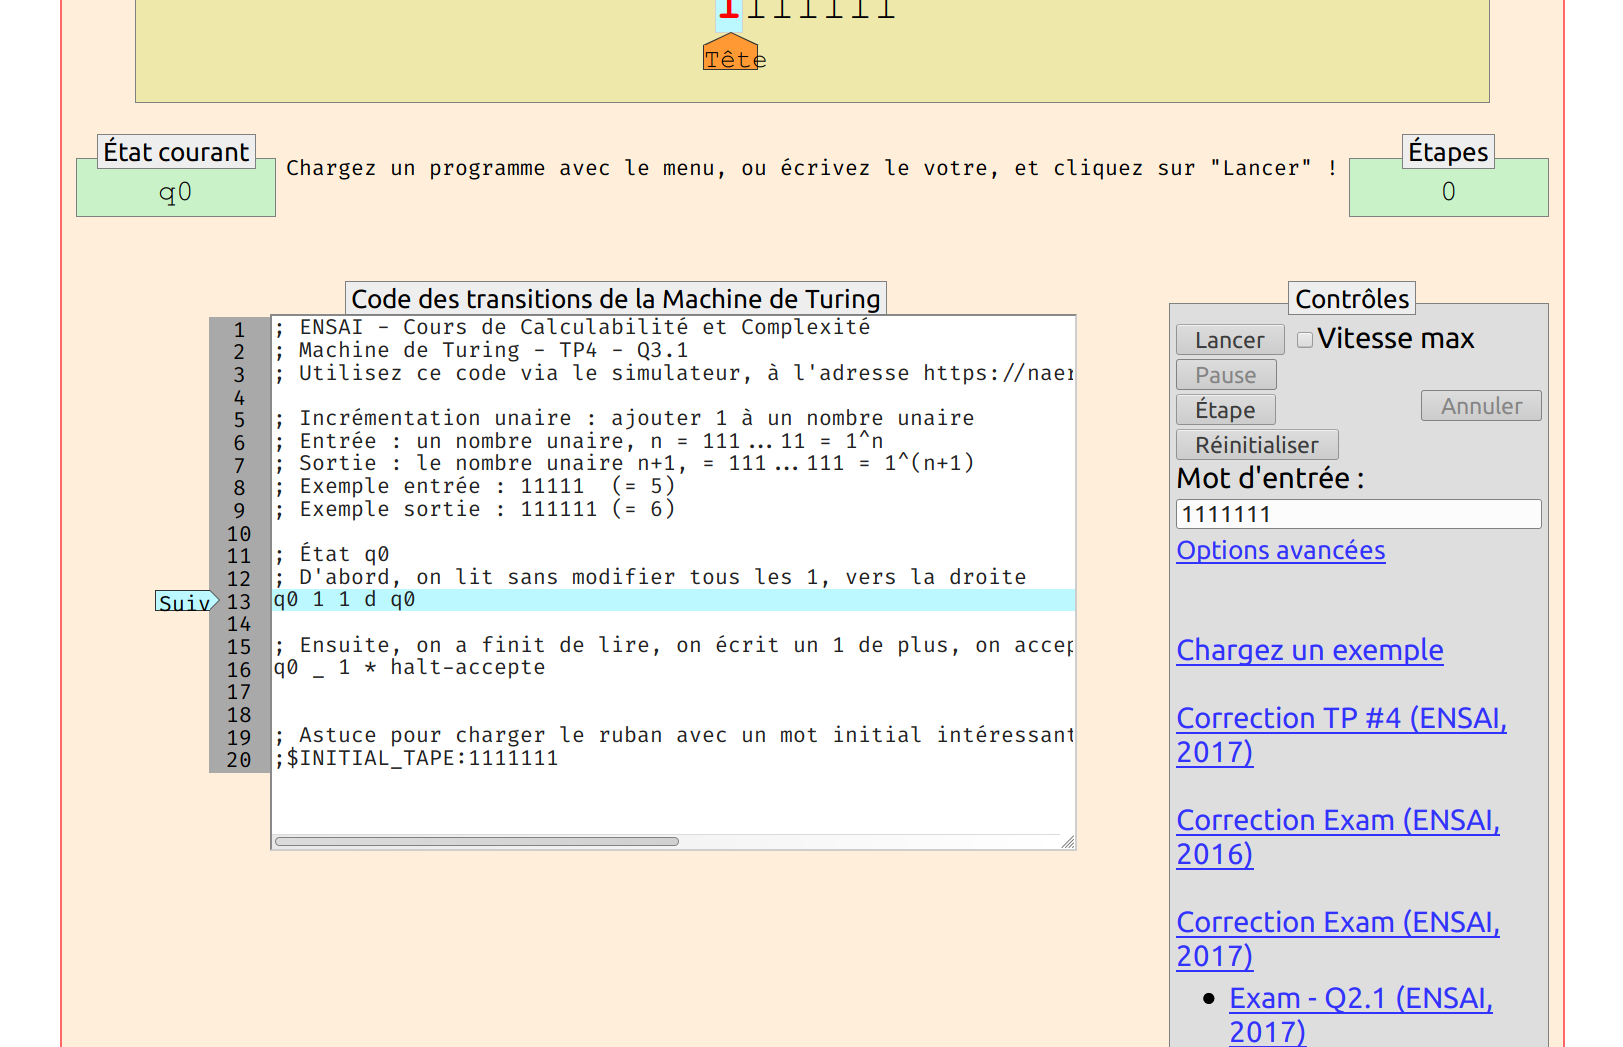
\includegraphics[width=9cm]{interactive_Turing_Machine_simulator_1.png}
    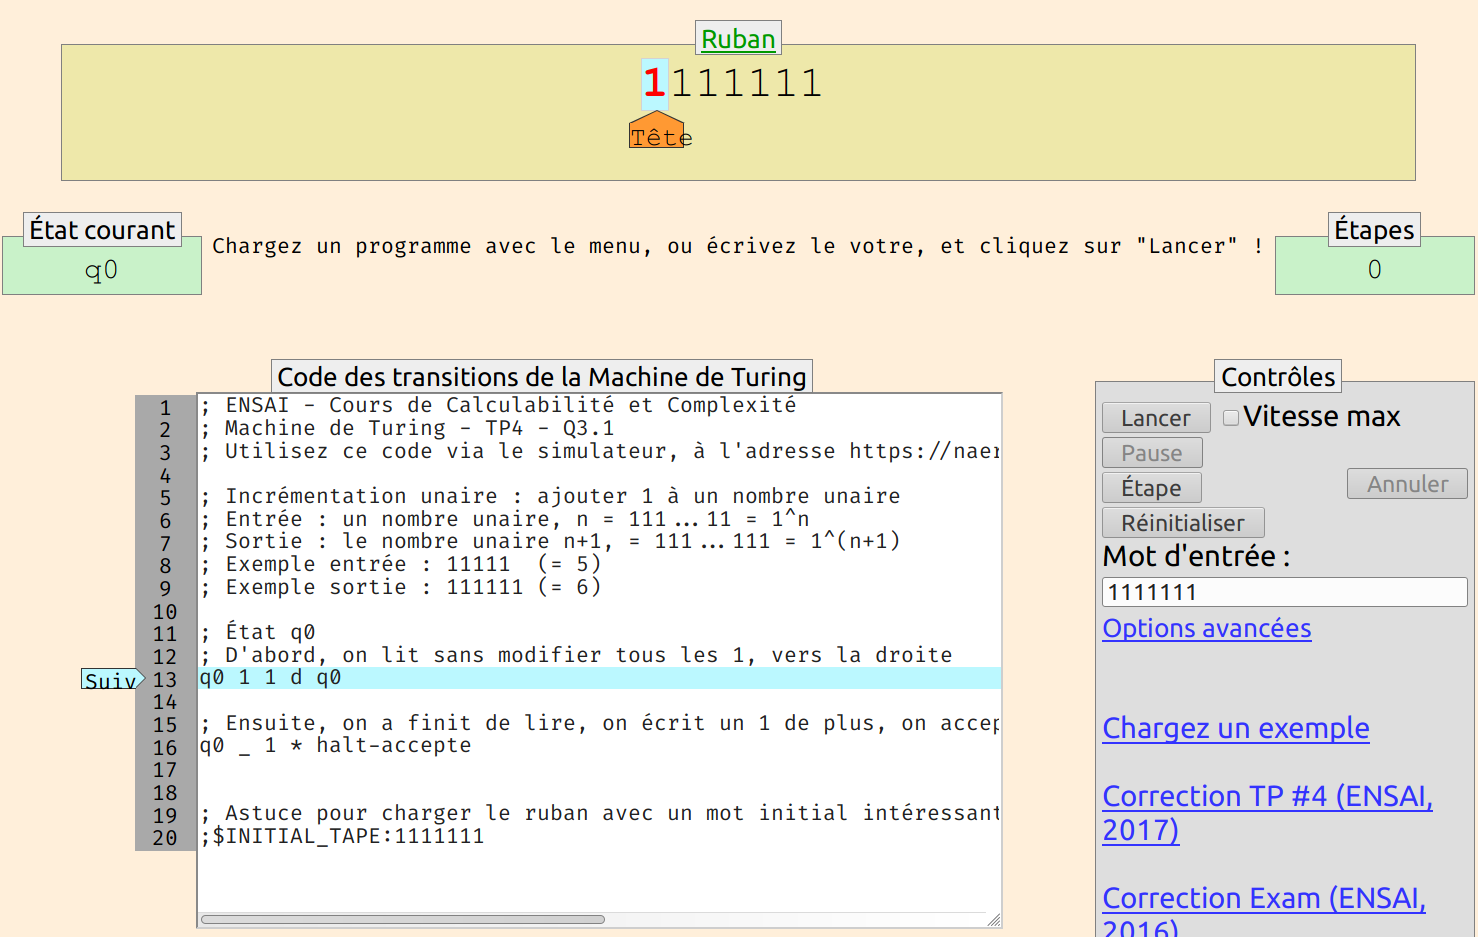
\includegraphics[width=9cm]{interactive_Turing_Machine_simulator_2.png}
    \caption{Screenshots of the user interface of the online Turing Machine simulator \url{https://naereen.github.io/jsTuring_fr/turing.html}.}
    % \label{}
\end{figure}


\paragraph{Use cases for teaching}

By allowing to load pre-written examples of Turing Machine, the simulator was successfully used in practical sessions for two different classes since 2017.


\paragraph{A curiosity: universal Turing Machine}

The last part of the poster will detail the interesting case of the universal Turing Machine, to tackle the most curious attendees of the conference.


% ---- Bibliography ----
%
% BibTeX users should specify bibliography style 'splncs04'.
% References will then be sorted and formatted in the correct style.
%
% \bibliographystyle{splncs04}
% \bibliography{mybibliography}
%
\begin{thebibliography}{8}
    \bibitem{turingmachine}
    Wikipedia contributors.
    \textbf{Turing Machine}, consulted in October 2019.
    \url{https://en.wikipedia.org/wiki/Turing_machine}.

    \bibitem{morphett_simulators}
    \textbf{Turing machine simulator},
    Anthony Morphett.
    Source code at \url{https://github.com/awmorp/jsturing},
    web interface at \url{http://morphett.info/turing/}.

    \bibitem{naereen_simulators}
    \textbf{Simulateur de Machines de Turing},
    Lilian Besson.
    Source code at \url{https://github.com/Naereen/jsTuring_fr},
    web interface at \url{https://naereen.github.io/jsTuring_fr/turing.html}.
\end{thebibliography}
\end{document}
